\documentclass{article}
\usepackage{tikz,pgfplots,tcolorbox}
\usetikzlibrary{arrows.meta,positioning,shapes,calc,decorations.pathreplacing,backgrounds,fit}
\pgfplotsset{compat=1.18}
\tcbuselibrary{skins,breakable}
\begin{document}
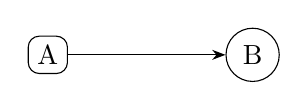
\begin{tikzpicture}[node distance=2cm]
\node[draw,rounded corners] (a) {A};
\node[draw,circle,right=of a] (b) {B};
\draw[-{Stealth}] (a) -- (b);
\end{tikzpicture}
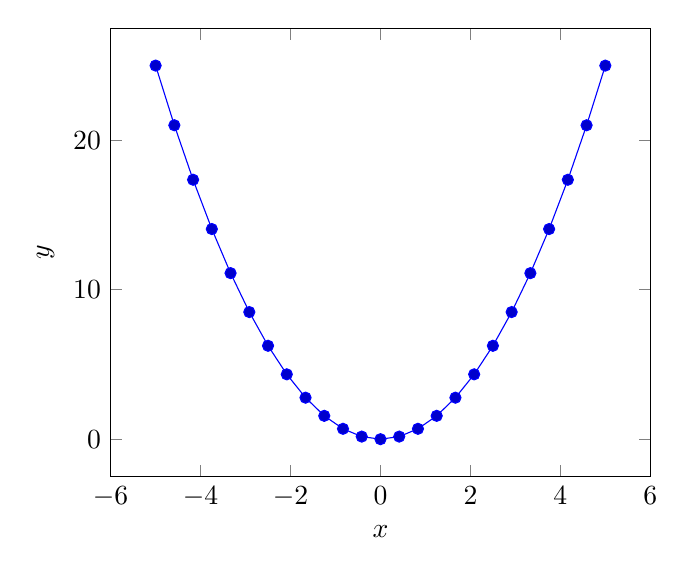
\begin{tikzpicture}\begin{axis}[xlabel=$x$,ylabel=$y$]\addplot {x^2};\end{axis}\end{tikzpicture}
\begin{tcolorbox}[title=Box,colback=blue!5]Content\end{tcolorbox}
\end{document}
